% Credits are indicated where needed. The general idea is based on a template by Vel (vel@LaTeXTemplates.com) and Frits Wenneker.

\documentclass[11pt, a4paper]{article} % General settings in the beginning (defines the document class of your paper)
% 11pt = is the font size
% A4 is the paper size
% “article” is your document class

%----------------------------------------------------------------------------------------
%	Packages
%----------------------------------------------------------------------------------------

% Necessary
\usepackage[german,english]{babel} % English and German language 
\usepackage{booktabs} % Horizontal rules in tables 
% For generating tables, use “LaTeX” online generator (https://www.tablesgenerator.com)
\usepackage{comment} % Necessary to comment several paragraphs at once
\usepackage[utf8]{inputenc} % Required for international characters
\usepackage[T1]{fontenc} % Required for output font encoding for international characters

% Might be helpful
\usepackage{amsmath,amsfonts,amsthm} % Math packages which might be useful for equations
\usepackage{tikz} % For tikz figures (to draw arrow diagrams, see a guide how to use them)
\usepackage{tikz-cd}
\usetikzlibrary{positioning,arrows} % Adding libraries for arrows
\usetikzlibrary{decorations.pathreplacing} % Adding libraries for decorations and paths
\usepackage{tikzsymbols} % For amazing symbols ;) https://mirror.hmc.edu/ctan/graphics/pgf/contrib/tikzsymbols/tikzsymbols.pdf 
\usepackage{blindtext} % To add some blind text in your paper
\usepackage{hyperref}


%---------------------------------------------------------------------------------
% Additional settings
%---------------------------------------------------------------------------------

%---------------------------------------------------------------------------------
% Define your margins
\usepackage{geometry} % Necessary package for defining margins

\geometry{
	top=2cm, % Defines top margin
	bottom=2cm, % Defines bottom margin
	left=2.2cm, % Defines left margin
	right=2.2cm, % Defines right margin
	includehead, % Includes space for a header
	%includefoot, % Includes space for a footer
	%showframe, % Uncomment if you want to show how it looks on the page 
}

\setlength{\parindent}{15pt} % Adjust to set you indent globally 

%---------------------------------------------------------------------------------
% Define your spacing
\usepackage{setspace} % Required for spacing
% Two options:
\linespread{1.5}
%\onehalfspacing % one-half-spacing linespread

%----------------------------------------------------------------------------------------
% Define your fonts
\usepackage[T1]{fontenc} % Output font encoding for international characters
\usepackage[utf8]{inputenc} % Required for inputting international characters

\usepackage{XCharter} % Use the XCharter font


%---------------------------------------------------------------------------------
% Define your headers and footers

\usepackage{fancyhdr} % Package is needed to define header and footer
\pagestyle{fancy} % Allows you to customize the headers and footers

%\renewcommand{\sectionmark}[1]{\markboth{#1}{}} % Removes the section number from the header when \leftmark is used

% Headers
\lhead{} % Define left header
\chead{\textit{}} % Define center header - e.g. add your paper title
\rhead{} % Define right header

% Footers
\lfoot{} % Define left footer
\cfoot{\footnotesize \thepage} % Define center footer
\rfoot{ } % Define right footer


%---------------------------------------------------------------------------------
%	General information
%---------------------------------------------------------------------------------
\title{Restaurant diversity in Boston neighborhods} % Adds your title
\author{
Brian Schaefer % Add your first and last name
    %\thanks{} % Adds a footnote to your title
    %\institution{YOUR INSTITUTION} % Adds your institution
  }

\date{\small \today} % Adds the current date to your “cover” page; leave empty if you do not want to add a date


%---------------------------------------------------------------------------------
%	Define what’s in your document
%---------------------------------------------------------------------------------

\begin{document}


% If you want a cover page, uncomment "\input{coverpage.tex}" and uncomment "\begin{comment}" and "\end{comment}" to comment the following lines
%\input{coverpage.tex}

%\begin{comment}
\maketitle % Print your title, author name and date; comment if you want a cover page 

%\end{comment}

%----------------------------------------------------------------------------------------
% Introduction
%----------------------------------------------------------------------------------------
\setcounter{page}{1} % Sets counter of page to 1

\section{Introduction}

Residents and frequent visitors of Boston are certainly familiar with its famous cultural centers and the food options each one provides.
Popular neighborhoods including Chinatown, North End, and the Seaport District are hot spots for those looking to indulge in the city's best Chinese, Italian, and seafood options.
But, where should one go for a more diverse selection of restaurants?
In this study, we classify neighborhoods in Boston based on restaurant variety and identify the neighborhoods with the most diverse options.

\section{Data}

To classify Boston's neighborhoods, we need geographical information about the neighborhoods as well as information on the types of restaurants that exist within each neighborhood.
For the former, we use geographical coordinates provided by the City of Boston outlining the boundaries of each of Boston's neighborhoods\footnote{\url{https://data.boston.gov/dataset/boston-neighborhoods}}.
For the latter, we use Foursquare\footnote{\url{https://www.foursquare.com}} to gather information on the types of restaurants nearby the geographical center of each neighborhood.

The geographical data are provided in \texttt{GeoJSON} format.
The dataset consists of multiple sets of \texttt{(longitude, latitude)} coordinates that define the boundaries of each neighborhood.
We adapt functions from the \texttt{geojson\_utils} Python package\footnote{\url{https://pypi.org/project/geojson_utils/}} to calculate the coordinates of the centroid and area of each neighborhood given the list of boundary coordinates.
Using the Python package \texttt{folium}, we can show the neighborhoods on an interactive map (Figure 1).

\begin{figure}
\begin{center}
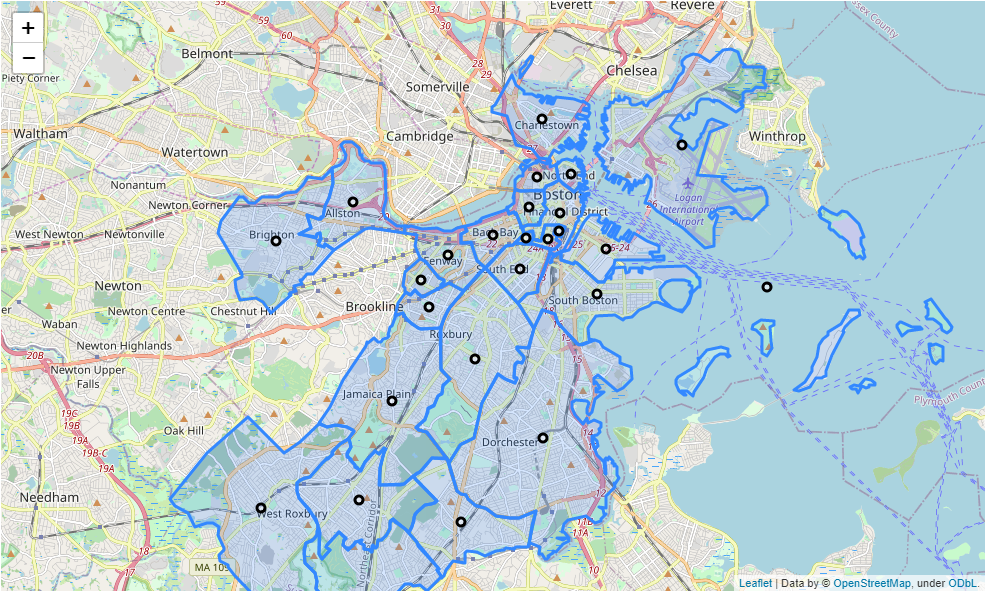
\includegraphics[width=0.7\textwidth]{folium_map.png}
\end{center}
\caption{Map of Boston neighborhoods (blue) and geographical centers (black markers).}
\end{figure}

We use the Foursquare application programming interface (API) to search for restaurants nearby each neighborhood's geographical center using the category ``Food''\footnote{\texttt{categoryId 4d4b7105d754a06374d81259}, \url{https://developer.foursquare.com/docs/build-with-foursquare/categories/}.}.
The Foursquare service returns the venue name, geographical coordinates, address, and category name for each of the ``Food'' venues found in the vicinity of each search point.
Since we are interested in unique types of restaurants in each neighborhood, we take the category name for each venue and ignore venues in the same neighborhood with the same name.
Figure 2 shows a summary of the relative frequencies of different types of venues across all neighborhoods. 
There are a few venue types that occur with very high frequency, and a relatively large number of unique venue types.

\begin{figure}
\begin{center}
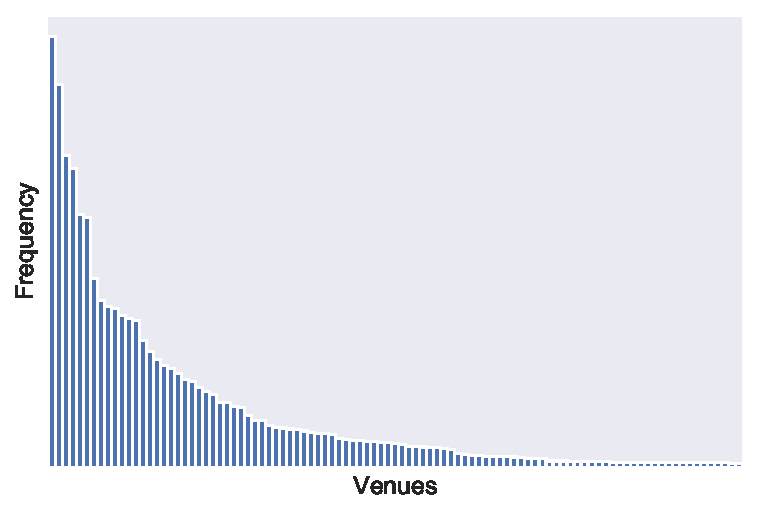
\includegraphics[width=0.5\textwidth]{summary_bar.pdf}
\end{center}
\caption{Frequency of venue types across all Boston neighborhoods.}
\end{figure}

\section{Methodology}

We seek to classify neighborhoods based on the number of diverse restaurant types.
If we simply count the number of different restaurant types, this will be biased towards neighborhoods that have many restaurants in total.
To account for this, we define a ``diversity index`` as follows:
$$
\text{Diversity} = \frac{\text{Number of unique restaurant types}}{\text{Total number of restaurants}}.
$$
We plot a histogram of this metric in Figure~3, and it appears that the neighborhoods in Boston vary significantly in terms of diversity.
The data approximately follow a normal distribution, with mean 0.61 and standard deviation 0.1.

\begin{figure}
\begin{center}
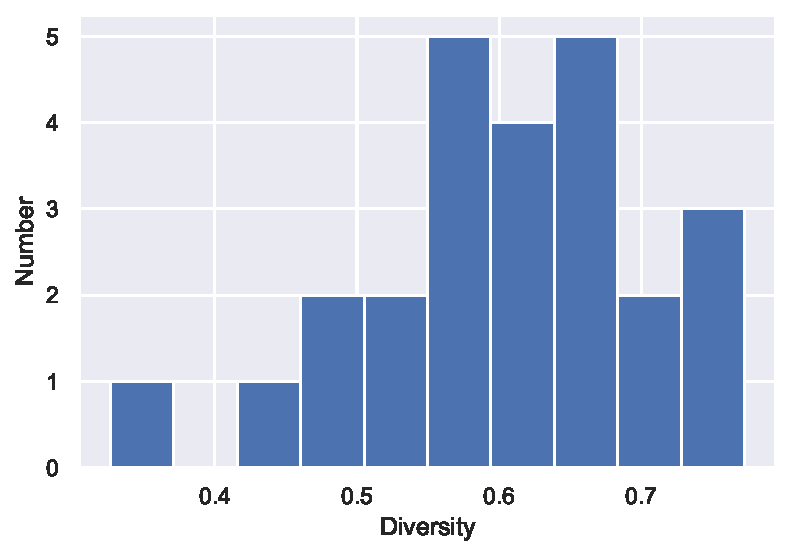
\includegraphics[width=0.5\textwidth]{diversity_hist.pdf}
\end{center}
\caption{Diversity index for Boston neighborhoods}
\end{figure}

To categorize the neighborhoods, we use the $k$-means clustering algorithm on a few different versions of the dataset.
This algorithm allocates data points into each of $k$ clusters by clustering together data points based on the similarity of the features for each data point.
The result of this algorithm is a cluster number assignment, ranging from $0...k$. 
We use the ``elbow'' method (Figure~4) to determine the optimal number of clusters.
By running the algorithm multiple times, with different number of clusters $k$ each time, we can understand how increasing the number of clusters can improve the algorithm's description of the data.
By eye, we choose the point of diminishing returns ($k$=3 in Figure~4) at which the rate of error improvement slows down (i.e., additional clusters do not provide useful information).


\begin{figure}
\begin{center}
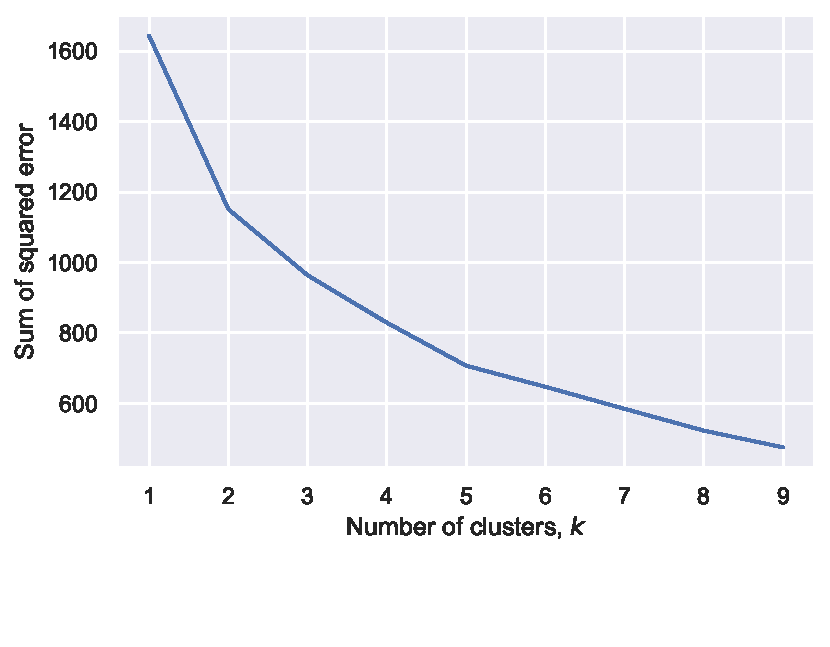
\includegraphics[width=0.5\textwidth]{elbow.pdf}
\end{center}
\caption{Elbow method for determining number of clusters}
\end{figure}


\section{Results}

We perform three clusterings of the neighborhoods, using (1) the total number of restaurants of each type in each neighborhood, (2) the proportion of restaurants of each type in each neighborhood, and (3) the diversity index for each neighborhood.

\subsection{Restaurant counts}
Using the Foursquare data, we total the numbers of restaurants labeled within each unique category name to arrive at a dataset of which we show in part below:
\begin{center}
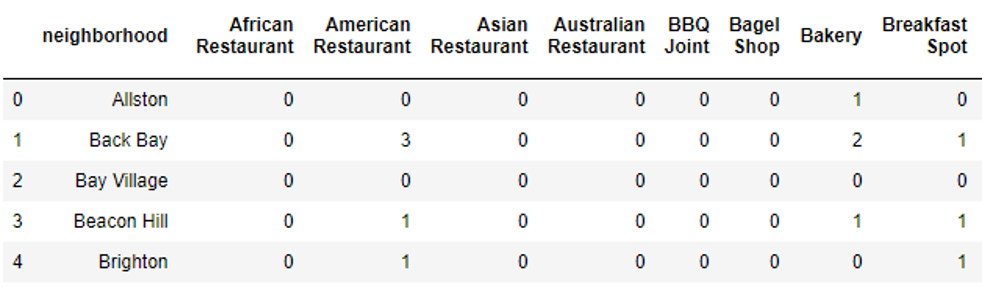
\includegraphics[]{df_counts.png}
\end{center}
For a given neighborhood (leftmost column), each data point is the number of restaurants falling into the category designated by the header above.
For example, in Back Bay there are three American Restaurants, two Bakeries, and one Breakfast Spot.

Performing $k$-means clustering to categorize the neighborhoods into three clusters, we find that the diversity index can vary substantially within each cluster (Figure~5).
The first two clusters have a diversity index ranging from $\sim0.4-0.7$, while the last cluster only has one neighborhood with a low diversity index.
Upon inspection of the most common restaurant types, we find that cluster 0 consists of neighborhoods with mainly pizza places and caf\'es, cluster 2 consists of the neighborhood with a preponderance of Italian restaurants (North End), while cluster 1 is more diverse.
This is a good start, as it correctly separates North End from the rest of the neighborhoods.
However, using just the count of restaurants of a given type does not account for the total number of restaurants.
\begin{figure}
\begin{center}
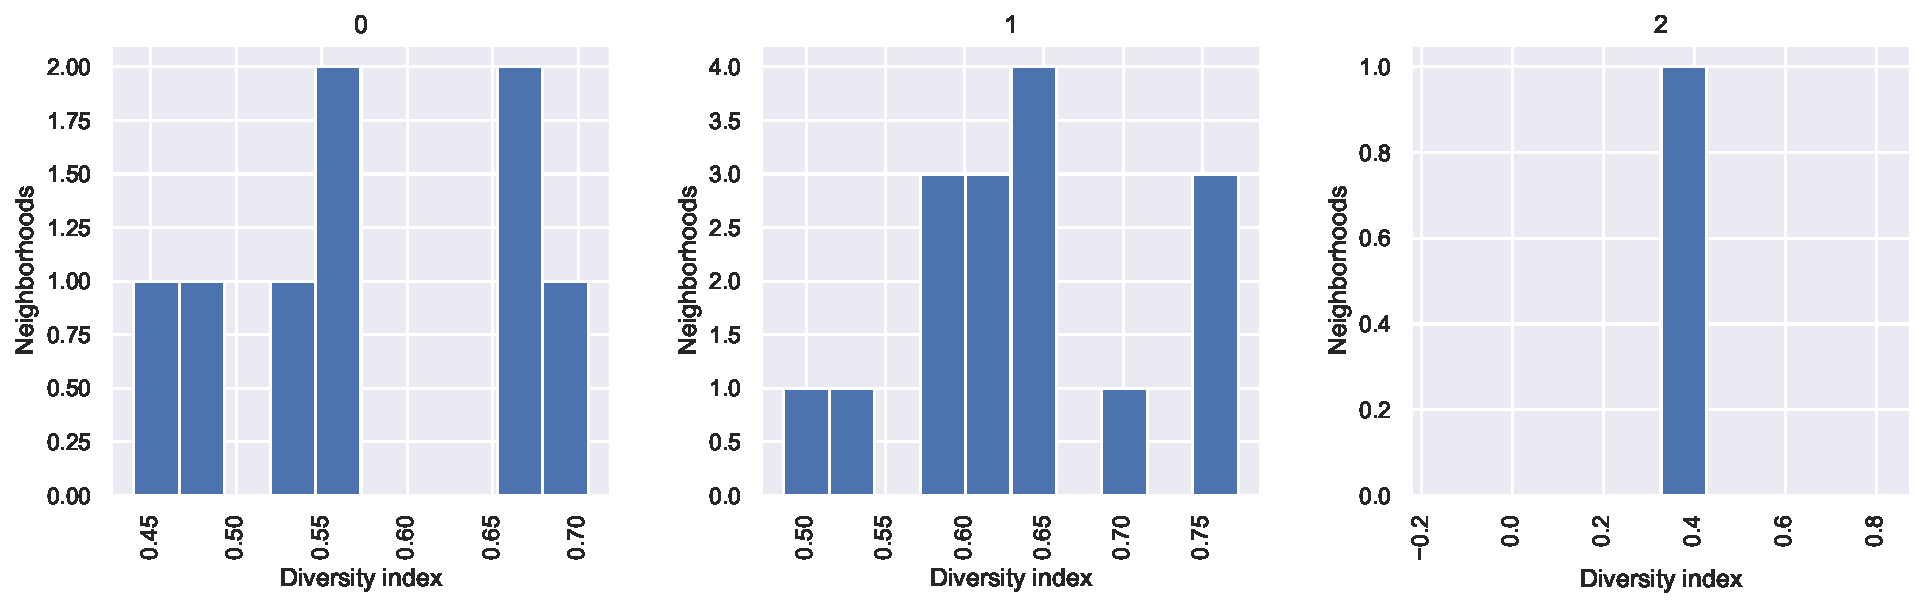
\includegraphics[width=\textwidth]{hist_counts.pdf}
\end{center}
\caption{Distribution of diversity index within each cluster, for clustering on data consisting of the counts of each restaurant type.}
\end{figure}



\subsection{Restaurant proportions}
By dividing each row of the dataset above by the total number of restaurants in each neighborhood, we get a dataset of the proportions of restaurants of each type:
\begin{center}
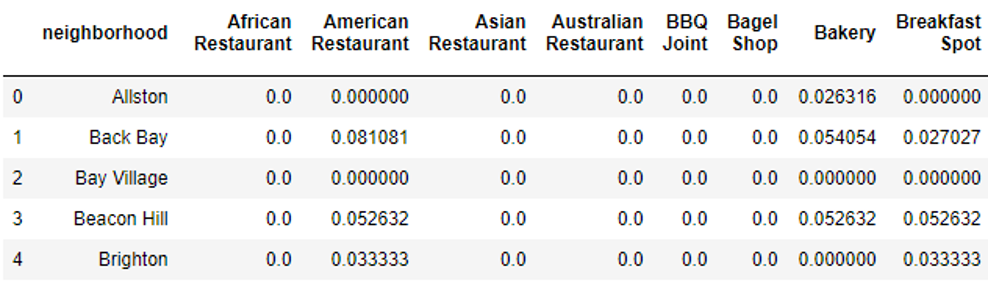
\includegraphics[]{df_prop.png}
\end{center}
For example, in Back Bay 8.1\% of restaurants are American Restaurants.


Performing $k$-means clustering to categorize the neighborhoods again into three clusters, we still see variance of the diversity index within each cluster (Figure~6).
Cluster 0 consists of North End and Bay Village, both of which have Italian restaurants as the most common type.
Cluster 1 again consists of neighborhoods with many pizza places and caf\'es, and cluster 2 is the most varied.
We are still not quite able to capture the clustering we want, so we move on to look only at the diversity index.
\begin{figure}
\begin{center}
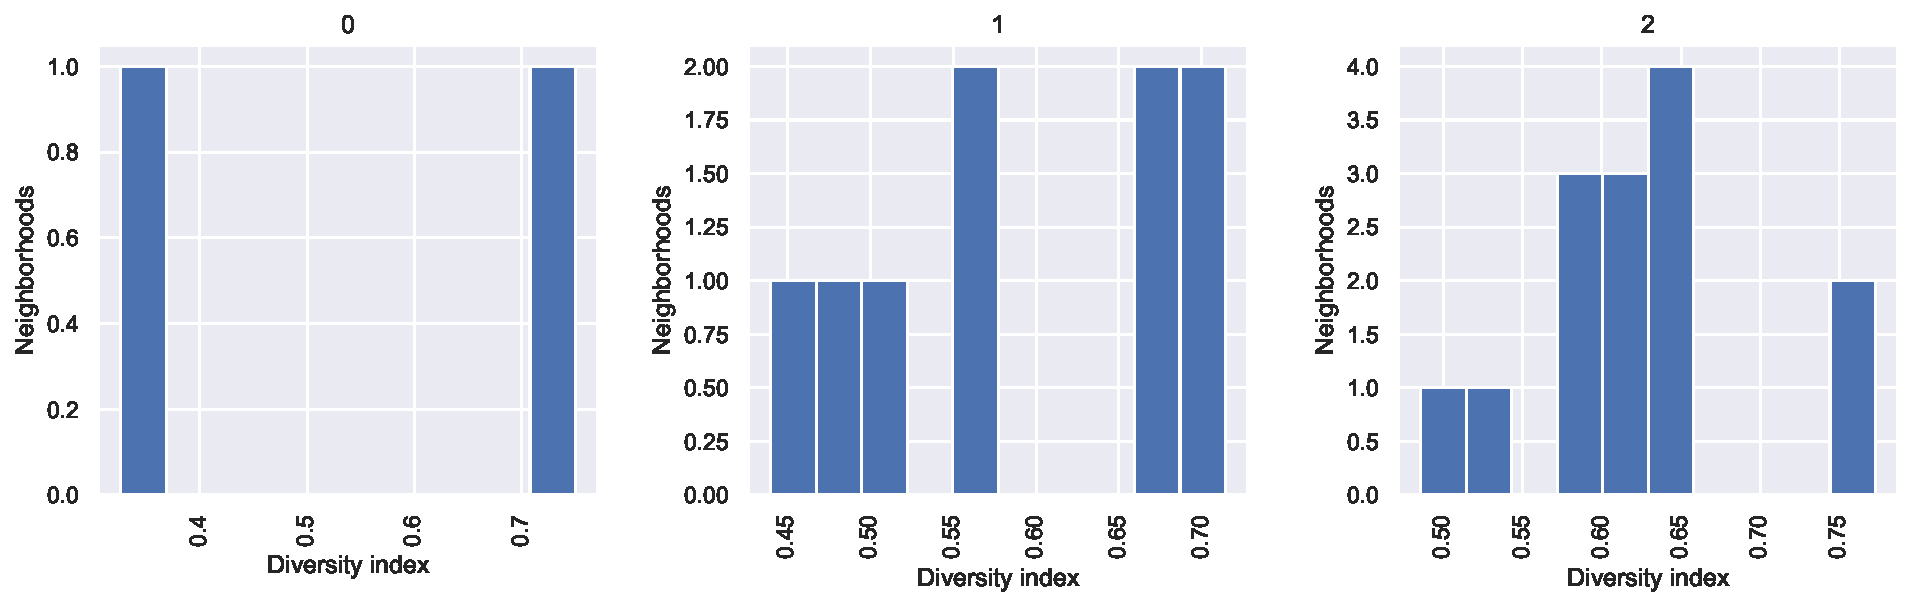
\includegraphics[width=\textwidth]{hist_prop.pdf}
\end{center}
\caption{Distribution of diversity index within each cluster, for clustering on data consisting of the proportion of each restaurant type.}
\end{figure}

\subsection{Diversity index}
We use the diversity index to form a much more limited dataset that already captures the gist of the question we set out to answer:
\begin{center}
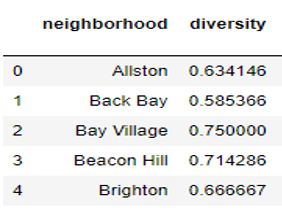
\includegraphics[]{df_diversity.png}
\end{center}

Performing $k$-means clustering, this time we find that each cluster contains an independent range of diversity index values (Figure~7).
Cluster 0 (diversity index $> 0.65$) is the most diverse, while cluster 2 (diversity index $<0.5$) is least diverse.
Table~1 summarizes the clustering.
The least diverse cluster now contains both Chinatown and North End, as expected for famous cultural centers.
The other two neighborhoods are unexpected, but make sense: Longwood is mainly a medical campus, which we would not expect to host diverse food options, and Mattapan has a large Afro-Caribbean influence, so many of the restaurants are expected to be Caribbean or African.

\begin{figure}
\begin{center}
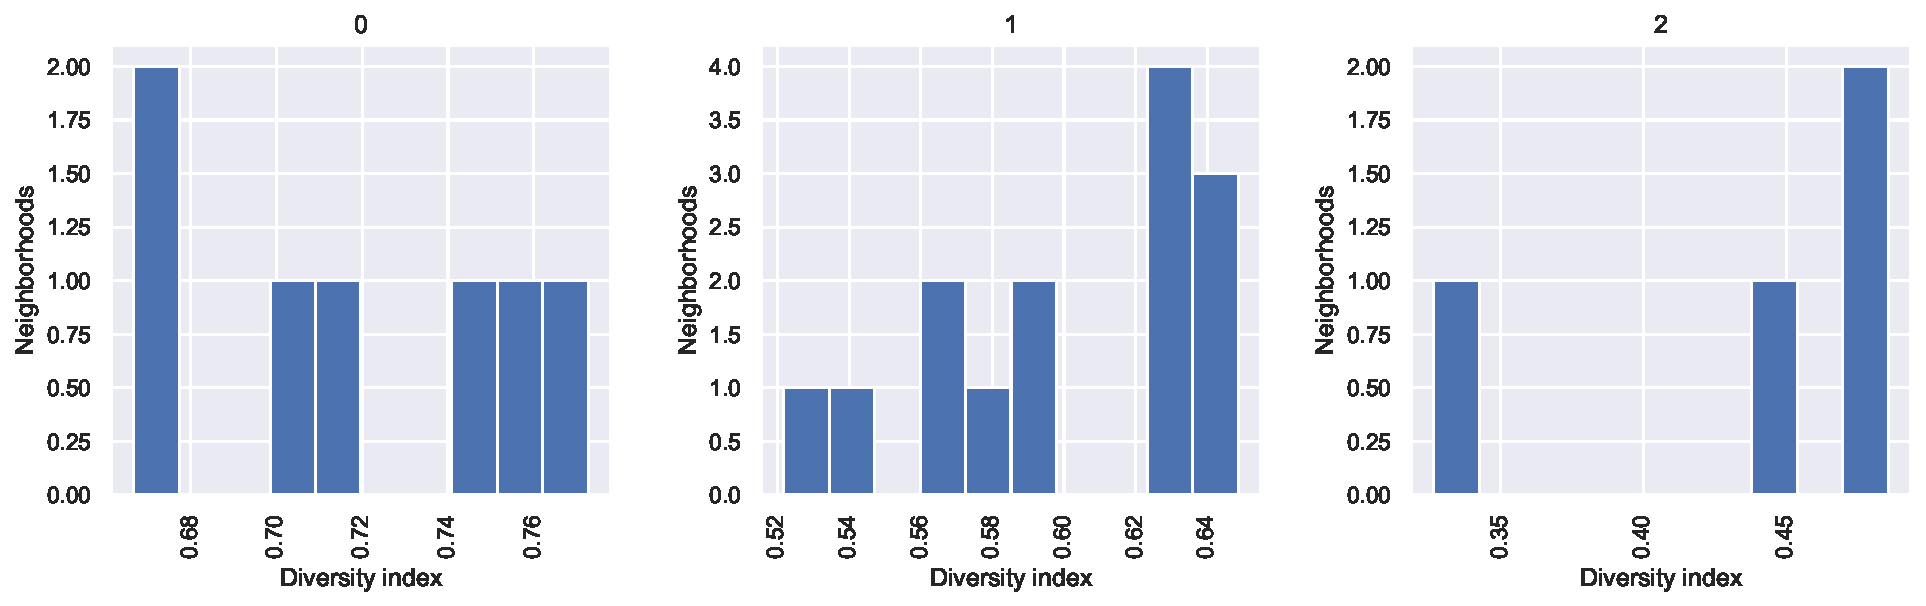
\includegraphics[width=\textwidth]{hist_diversity.pdf}
\end{center}
\caption{Distribution of diversity index within each cluster, for clustering on only the diversity index.}
\end{figure}

\begin{table}[]
\begin{center}
\begin{tabular}{| l | l |}
\hline
Cluster 0 & Bay Village, Beacon Hill, Brighton, Mission Hill, ... \\
\hline
Cluster 1 & Allston, Back Bay, Charlestonwn, Dorchester, ...      \\
\hline
Cluster 2 & Chinatown, North End, Longwood, Mattapan     \\        
\hline
\end{tabular}
\end{center}
\caption{Neighborhoods clustered on diversity index}
\end{table}

\section{Discussion}

The final clustering of neighborhoods makes sense based on common knowledge of Boston's most famous neighborhoods.
Are there any patterns in the geographical location of the most diverse food neighborhoods in Boston?
In Figure~8, we show a map of the neighborhoods color-coded by cluster.
Interestingly, we notice a string of three diverse neighborhoods on the west side of the city center, while the neighborhoods on the east side are less diverse.
We also notice a few diverse neighborhoods further from the city center.

\begin{figure}
\begin{center}
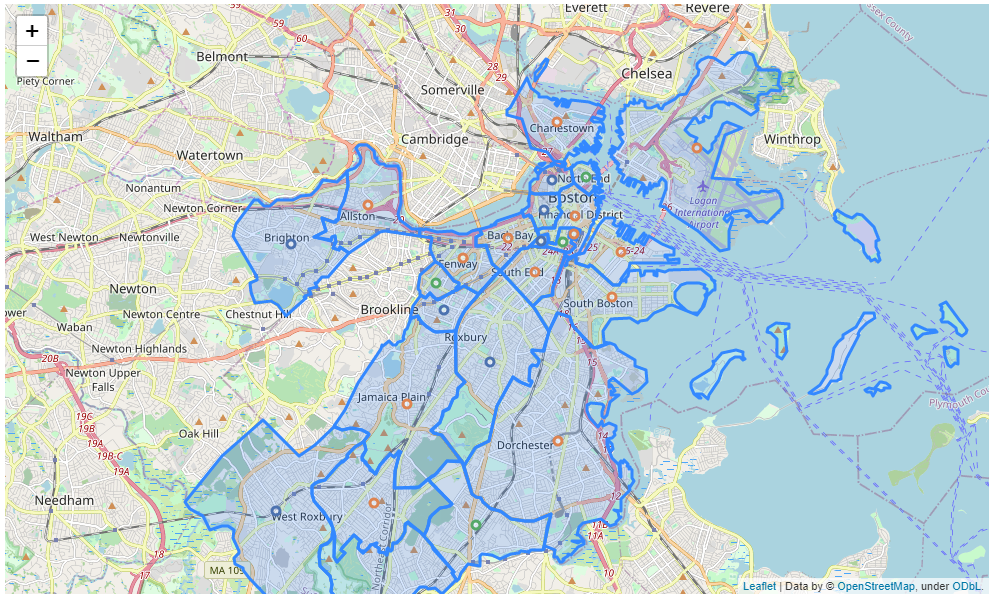
\includegraphics[width=0.7\textwidth]{final_clustering.png}
\end{center}
\caption{Map of Boston neighborhoods (blue outlines) and geographical centers sorted by cluster (green: least diverse, orange: moderately diverse, dark blue: most diverse).}
\end{figure}

\section{Conclusion}
We clustered neighborhoods in Boston based on the diversity of the restaurants nearby the geographical centers of each neighborhood.
As expected, famous cultural centers like Chinatown and North End are deemed some of the least diverse cities, while other neighborhoods like Back Bay are deemed much more diverse.
We have compiled a list of neighborhoods offering a variety of dining options that would be great spots for both visitors and new residents to Boston with an adventurous palate.


%---------------------------------------------------------------------------------

\end{document}